%\iffalse
\let\negmedspace\undefined
\let\negthickspace\undefined
\documentclass[journal,12pt,twocolumn]{IEEEtran}
\usepackage{cite}
\usepackage{amsmath,amssymb,amsfonts}
\usepackage{graphicx}
\usepackage{textcomp}
\usepackage{xcolor}
\usepackage{txfonts}
\usepackage{listings}
\usepackage{enumitem}
\usepackage{mathtools}
\usepackage{gensymb}
\usepackage{comment}
\usepackage[breaklinks=true]{hyperref}
\usepackage{tkz-euclide} 
\usepackage{listings}
\usepackage{gvv}                                        
\def\inputGnumericTable{}                                 
\usepackage[latin1]{inputenc}                                
\usepackage{color}                                            
\usepackage{array}                                            
\usepackage{longtable}                                       
\usepackage{calc}                                             
\usepackage{multirow}                                         
\usepackage{hhline}                                           
\usepackage{ifthen}                                           
\usepackage{lscape}
\usepackage[export]{adjustbox}

\newtheorem{theorem}{Theorem}[section]
\newtheorem{problem}{Problem}
\newtheorem{proposition}{Proposition}[section]
\newtheorem{lemma}{Lemma}[section]
\newtheorem{corollary}[theorem]{Corollary}
\newtheorem{example}{Example}[section]
\newtheorem{definition}[problem]{Definition}
\newcommand{\BEQA}{\begin{eqnarray}}
\newcommand{\EEQA}{\end{eqnarray}}
\newcommand{\define}{\stackrel{\triangle}{=}}
\newtheorem{rem}{Remark}

\begin{document}
\parindent 0px
\bibliographystyle{IEEEtran}

\vspace{3cm}

\title{GATE:EE/63}
\author{EE23BTECH11208 - Manohar K$^{*}$
}
\maketitle
\newpage
\bigskip

% \renewcommand{\thefigure}{\theenumi}
% \renewcommand{\thetable}{\theenumi}



\textbf{Question:} \hspace{2pt} A signal $x\brak{t}=2\cos{(180\pi t)}\cos{(60\pi t)}$ is sampled at 200 Hz and then passed through an ideal low pass filter having cut-off frequency of 100 Hz.\\
The maximum Frequency present in the filtered  signal in Hz is \rule{1cm}{0.5mm} (Round off to the nearest integer.) \hfill (GATE 2023 EE)\\
\noindent \textbf{Solution:}\\
\begin{figure}[ht]
	\centering
	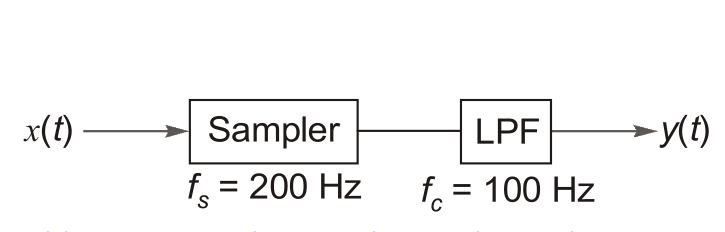
\includegraphics[width=1\linewidth]{figs/answerdia.png}
\end{figure}
Given, \\

\begin{align}
	x\brak{t}&=cos\brak{240\pi t} + cos\brak{120\pi t}
\end{align}
\begin{table}[h]
	\centering
	
\begin{tabular}{|c|c|}
	\hline
	\textbf{symbol} & \textbf{description} \\
	\hline
	$G$ & Forward path gain\\
	\hline
	$H$ & Feedback path gain\\
	\hline
	$R(s)$ & Input signal \\
	\hline
	$C(s)$ & Output signal \\
	\hline
	$E(s)$ & Error signal \\
	\hline
\end{tabular}
	\caption{Parameters}
	\label{tab:GATE.EE.2023.63}
\end{table}
\begin{align}
	& f_1 , (f_s\pm f_1) , (2f_s \pm f_1) \dots\\
	& 120, 80,340,280,520 \dots\\
	& f_2 , (f_s\pm f_2) , (2f_s\pm f_2) \dots\\
	& 60 , 140,260,34,460 \dots 
	 \end{align}
From table $f_c = 100Hz$ \\
LPF output : $60Hz$ , $80Hz$\\
Maximum Frequency present in the filtered signal is $80Hz$

\begin{figure}[ht]
	\centering
	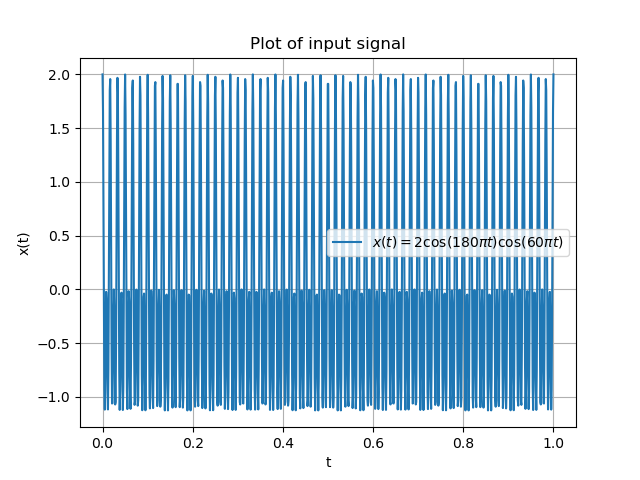
\includegraphics[width=1\linewidth]{figs/signalplot.png}
	\caption{Plot of x(t) vs t}
\end{figure}
\begin{figure}[ht]
	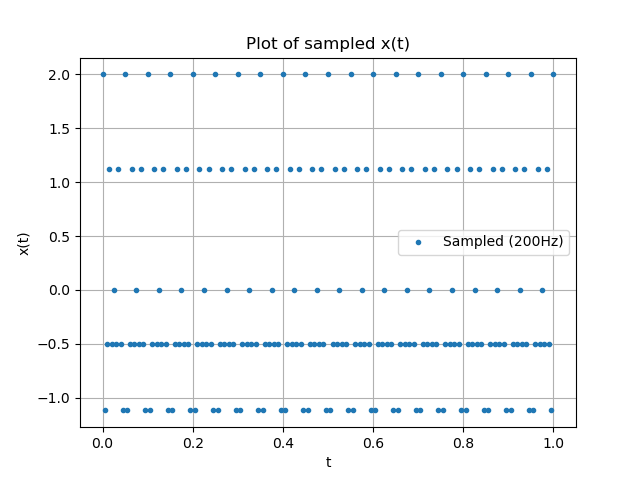
\includegraphics[width=1\linewidth]{figs/samplingplot.png}
	\caption{Plot of x(t) vs t}
\end{figure}
\end{document}
